\section{Theorie}
\label{sec:Theorie}
Im Folgenden werden die Grundlagen der Vakuumtechnik erklärt, sowie einige Begriffe definiert. Diese Informationen stammen, falls nicht explizit anders angegeben, von Pfeiffer Vacuum\cite{Pfeiffer}.
\subsection{Vakuum}
Ein Vakuum ist ein Volumen, das frei von Materie ist. In der Umgangssprache ist damit oft ein luftleer Raum gemeint, in wissenschaftlichen Sinne sind aber auch
andere Gase oder Partikel gemeint. Da es nicht möglich ist ein perfektes Vakuum zu erstellen, wird zwischen verschiedenen Güteklassen unterschieden. Diese
unterscheiden sich in ihrem Unterdruck, also dem Druckunterschied zum Normaldruck. Es werden die folgenden Klassen von Vakua unterschieden.
\begin{description}
	\item[Normaldruck] $\SI{1013.25}{\milli \bar}$
	\item[Grobvakuum] $\SI{300}{\milli \bar}$
	\item[Feinvakuum] $\SI{1}{\milli \bar}$ bis $\SI{e-3}{\milli \bar}$
	\item[Hochvakuum (HV)] $\SI{e-3}{\milli \bar}$ bis $\SI{e-7}{\milli \bar}$
	\item[Ultrahochvakuum (UHV)] $\SI{e-7}{\milli \bar}$ bis $\SI{e-12}{\milli \bar}$
	\item[extrem hohes Vakuum (XHV)] < $\SI{e-12}{\milli \bar}$
	\item[ideales Vakuum (IV)] $\SI{0}{\milli \bar}$
\end{description}
\subsection{Gasphysik}
Die einfachste Besceschreibung für Gase ist die ideale Gasgleichung:
\begin{equation}
	pV=Nk_\text{B}T
\end{equation}
Diese gilt, wenn das Gas aus identischen Teilchen ohne Ausdehnung besteht, diese nur über elastische Stöße wechselwirken und das Gas in einem Volumen $V$ eingeschlossen
ist, mit dessen Begrenzung auch nur elastisch gestoßen wird. Aus dieser Formel ist auch ersichtlich, dass $p=0$ nicht möglich ist, da dann $T=0$ gelten
müsste, was nach dem 3. Hauptsatz der Thermodynamik unerreichbar ist. Es lässt sich auch das Gesetz von Boyle-Mariotte herleiten, das besagt, dass bei
 konstanter Temperatur der Druck $p$ antiproportional zu $V$ ist. Zudem kann zu der Teilchendichte umgestellt werden.\cite{TuSKierfeld}
 \begin{equation}
 	\frac{N}{V}=\frac{k_\text{B}T}{p}
 \end{equation}

\subsection{Druck}
Der Druck gibt die Kraft an, die ein Gas auf sein Behältnis ausübt. Er wird in $\si{\pascal}=\si{\newton \per \meter \squared}$ gemessen, oft wird aber auch die Einheit $1 \si{\bar}=\SI{100}{\pascal}$ verwendet. Falls ein Gasgemisch
vorliegt, steht jeder Gasanteil unter einem Partialruck $p_i$.
\subsection{Mittlere freie Weglänge}
Die mittlere freie Weglänge gibt an, wie weit ein Teilchen sich statistisch bewegen kann, bis es mit einem anderen Teilchen wechselwirkt.
Sie wird von der Formel
\begin{equation}
	l=\frac{k_\text{B}T}{\sqrt{2}\pi p d^2}
\end{equation}
beschrieben. Hierbei ist $d$ der Moleküldurchmesser.

\subsection{Drehschieberpumpe}
Eine Drehschieberpumpe besteht aus einem zylindrischen Hohlraum, in dem exzentrisch ein Rotor gelagert ist. An diesem Rotor sind zwei oder drei Drehschieber,
die durch eine Feder den variablen Abstand zur Außenwand abschließen. Der Pumpeneinzug ist mit dem großen Volumen befestigt, der Ausstoß mit dem Kleinen.
Wenn der Rotor nun gedreht wird, strömt Gas in die große Kammer ein. Dieses Gas wird dann von dem nachfolgenden Drehschieber isoliert. Das eingeschlossene Gas wird
durch die Drehung immer weiter komprimiert, bis der Überdruck ausreicht um das Auslassventil zu öffnen. Der Aufbau ist in Abbildung \ref{img:drehpump} zu sehen.
\begin{figure}
	\centering
	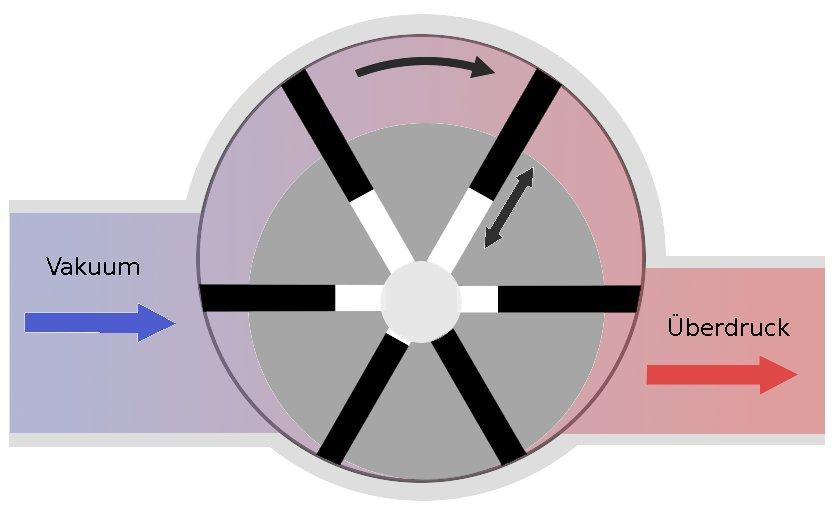
\includegraphics[width=0.8\textwidth]{img/drehpump.jpg}
	\caption{Schematischer Aufbau einer Drehschieberpumpe.\cite{hoechs}}
	\label{img:drehpump}
\end{figure}
\subsection{Turbomolekularpumpe}
Eine Turbomolekularpumpe besteht aus einem Hohlzylinder, in dem abwechselnd Rotoren und Statoren sind. Dabei sind die Rotorblätter in Drehrichtung und die
Statorblätter in die entgegengesetzte Richtung gekippt. Wenn nun ein Molekül einen Rotor trifft, wird es in Drehrichtung beschleunigt. Das darauf folgende Stratorblatt lenkt das Molekül dann
in den nächsten Rotor. Es ist für die Funktionsweise wichtig, dass Geschwindigkeit der Rotorblätter größer ist als die mittlere Molekülgeschwindigkeit des
Gases. Zudem müssen die Abstände der Rotoren in der Größenordnung der mittleren freien Weglänge der Gasmoleküle liegen, da die Bewegung sonst zum Erliegen
kommt. Der Aufbau ist in Abbildung \ref{img:turbopump} zu sehen.
\begin{figure}
	\centering
	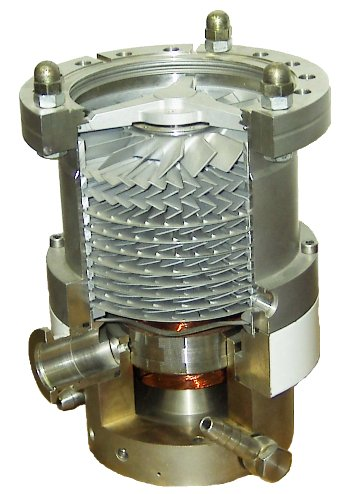
\includegraphics[width=0.8\textwidth]{img/turbopump.jpg}
	\caption{Schematischer Aufbau einer Turbomolekularpumpe.\cite{wiki}}
	\label{img:turbopump}
\end{figure}
\subsection{Vakuummeter}
\subsubsection{Kalt-/Glühkathoden}
Bei diesem Vakuummeter wird zwischen einer Kathode und einer Anode eine Spannung von ca $\SI{2}{\kilo \volt}$ angelegt. Dadurch werden Elektronen
beschleunigt, die auf ihrem Weg mit Gasteilchen stoßen und diese ionisieren. Diese Gas-Ionen werden zu der Kathode beschleunigt und es lässt sich ein
Strom messen. Dieser ist abhängig von dem Druck bzw. der Anzahl an Stößen, die ausgeführt werden. Es wird unterschieden zwischen Kaltkathoden, bei den bereits
vorhandene Elektronen beschleunigt werden, und Glühkathoden, bei denen mit dem glühelektrischen Effekt Elektronen aus der Kathode ausgelöst werden.
\subsubsection{Pirani-Vakuummeter}
Beim Pirani-Vakuummeter wird die Abhängigkeit der Wärmeleitfähigkeit vom Druck ausgenutzt. Dazu wird ein Draht elektrisch erwärmt. Dieser gibt ein Teil der
Wärmeenergie an das ihn umgebene Gas ab, der Rest staut sich im Draht auf. Da bei niedrigeren Druck die Wärmeleitung abnimmt, wird der Draht umso wärmer, je
geringer der Umgebungsdruck ist. Die Temperatur des Drahtes kann über den elektrischen Wiederstande gemessen werden.
\subsection{Lecks}
Ein Vakuum kann reale und virtuelle Lecks haben. Bei realen Lecks kann Gas von außerhalb des Aufbaus in den Rezipienten eindringen, zum Beispiel durch
nicht richtig abgedichtete Flansche. Diese Lecks kann man einfach abdichten, wenn man sie lokalisiert hat. Bei virtuellen Lecks strömen Teilchen aus dem
Aufbau selbst in den Rezipienten, zum Beispiel Einschlüsse in Metallteilen. Diese lassen sich in den meisten Fällen nicht abdichten, sondern müssen schon
bei der Produktion vermieden werden.
\subsection{Generelle Definitionen}
Im Folgenden werden einige Fachbegriffe aus der Vakuumtechnik erläutert.
\begin{description}
	\item[Absorbtion] Aufnahme eines Teilchens in einen Festkörper
	\item[Adsorbtion] Ablagerung eines Teilchens auf der Oberfläche eines Festkörpers
	\item[Desorbtion] Ablösen eines Teilchens von der Oberfläche eines Festkörpers
	\item[Diffusion] Vermischung von Gasen bzw. Flüssigkeiten durch Molekularbewegung
	\item[Laminare Stömung] Wirbelfreie Strömung
	\item[Saugleistung] $\dot{Q}$, Stoffmenge pro Zeit
\end{description}
\subsection{Leitwert}
Nur sehr selten wird eine Pumpe direkt an einen Versuchaufbau angeschlossen. In der Regel wird ein Schlauchsystem eingesetzt. Dieses hat neben der Volumensvergrößerung
noch mehr negative Auswirkungen auf das reale Saugvermögen der Pumpe. Es entsteht ein Druckgefälle zur Pumpe hin, bedingt durch den Strömungswiderstand des Schlauchsystems. In der Regel wird der Kehrwert dieses Widerstands benutzt: der Leitwert. Der Leitwert verhält sich analog zu $\sfrac{1}{R}$ in elektrischen
Systemen:
\begin{align}
	L_\text{ges, parallel}=&\sum_i L_i \\
	L_\text{ges, reihe}=&\sum_i \frac{1}{L_i}.
\end{align}
